\begin{figure*}[!htb]

    \begin{subfigure}[b]{0.45\textwidth}
        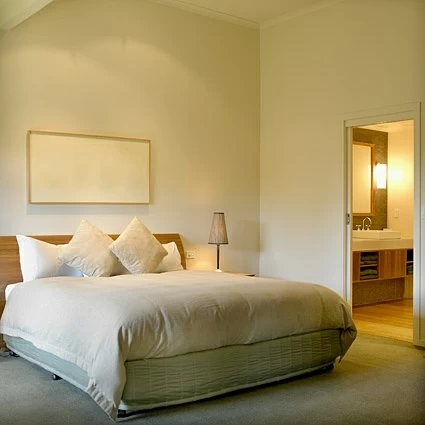
\includegraphics[width=\textwidth]{figures/bedroom/original_sample.png}
    \end{subfigure}
    \begin{subfigure}[b]{0.45\textwidth}
        \subfloat{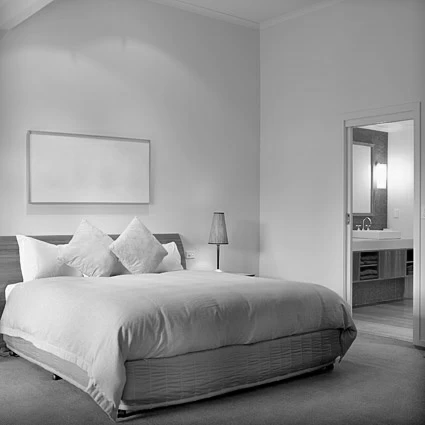
\includegraphics[height=0.33\textwidth]{figures/bedroom/greyscale_sample.png}}\hfill
        \subfloat{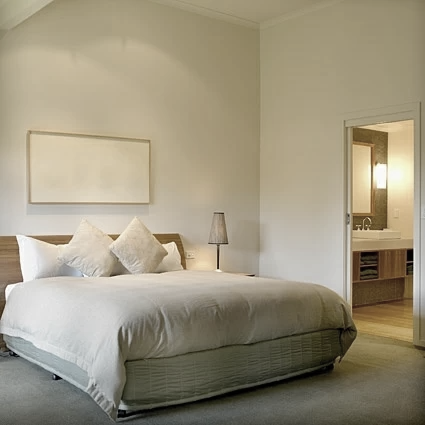
\includegraphics[height=0.33\textwidth]{figures/bedroom/desaturated_sample.png}}\hfill
        \subfloat{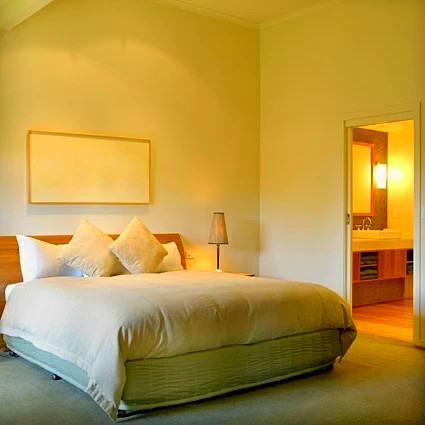
\includegraphics[height=0.33\textwidth]{figures/bedroom/Sat.png}}\hfill
        \subfloat{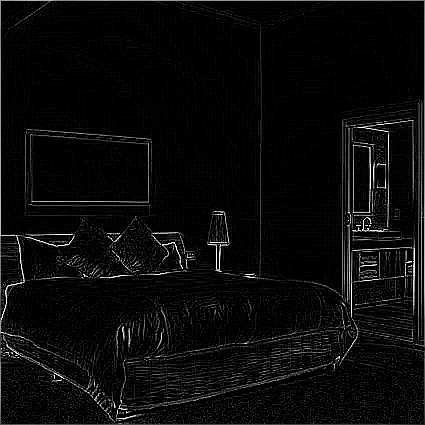
\includegraphics[height=0.33\textwidth]{figures/bedroom/edge_sample.png}}\hfill
        \subfloat{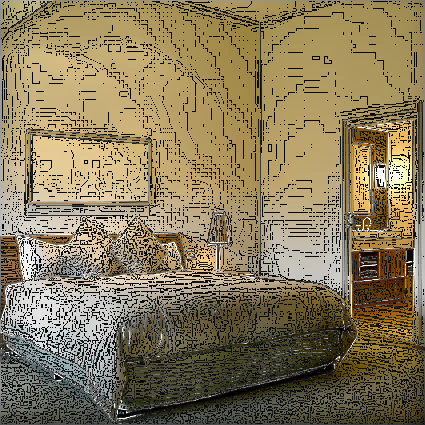
\includegraphics[height=0.33\textwidth]{figures/bedroom/EdgeCol5.png}}\hfill
        \subfloat{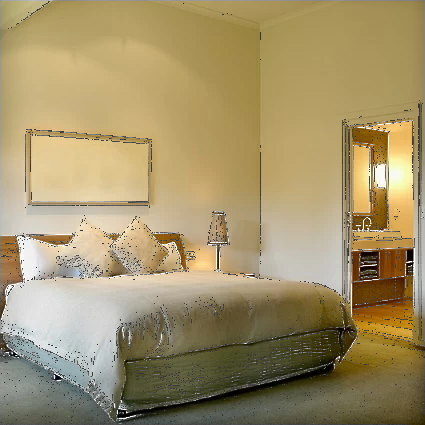
\includegraphics[height=0.33\textwidth]{figures/bedroom/EdgeCol50.png}}\hfill
        \subfloat{
\includegraphics[width=0.33\textwidth]{figures/bedroom/ih6no69aj90y-400747926.png}}\hfill
        \subfloat{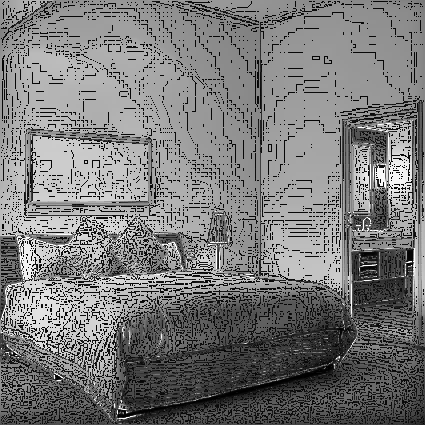
\includegraphics[height=0.33\textwidth]{figures/bedroom/greyscale_edge_s_sample.png}} \hfill
        \subfloat{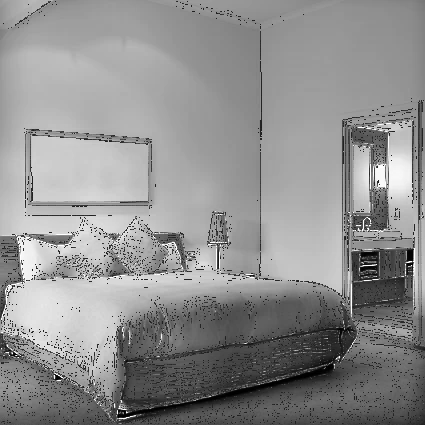
\includegraphics[height=0.33\textwidth]{figures/bedroom/greyscale_edge_sample.png}}
        
         
    \end{subfigure}
    \label{fig:samples}
    
    \caption{Different Data augmentation methods applied on the sample image which can be seen on the left. The images were augmented  from left to write int the following ways: (a) Greyscaled, (b) Desaturated, (c) Oversaturated, (d) Edge Detection, (e) Colour Image overlayed with edges with $>2\%$ white value, (f) Colour Image overlayed with edges with $>20\%$ white value, (g) Greyscaled Image overlayed with edges with $>2\%$ white value and (h) Greyscaled Image overlayed with edges with $>20\%$ white value}
\end{figure*}